\documentclass[1p]{elsarticle_modified}
%\bibliographystyle{elsarticle-num}

%\usepackage[colorlinks]{hyperref}
%\usepackage{abbrmath_seonhwa} %\Abb, \Ascr, \Acal ,\Abf, \Afrak
\usepackage{amsfonts}
\usepackage{amssymb}
\usepackage{amsmath}
\usepackage{amsthm}
\usepackage{scalefnt}
\usepackage{amsbsy}
\usepackage{kotex}
\usepackage{caption}
\usepackage{subfig}
\usepackage{color}
\usepackage{graphicx}
\usepackage{xcolor} %% white, black, red, green, blue, cyan, magenta, yellow
\usepackage{float}
\usepackage{setspace}
\usepackage{hyperref}

\usepackage{tikz}
\usetikzlibrary{arrows}

\usepackage{multirow}
\usepackage{array} % fixed length table
\usepackage{hhline}

%%%%%%%%%%%%%%%%%%%%%
\makeatletter
\renewcommand*\env@matrix[1][\arraystretch]{%
	\edef\arraystretch{#1}%
	\hskip -\arraycolsep
	\let\@ifnextchar\new@ifnextchar
	\array{*\c@MaxMatrixCols c}}
\makeatother %https://tex.stackexchange.com/questions/14071/how-can-i-increase-the-line-spacing-in-a-matrix
%%%%%%%%%%%%%%%

\usepackage[normalem]{ulem}

\newcommand{\msout}[1]{\ifmmode\text{\sout{\ensuremath{#1}}}\else\sout{#1}\fi}
%SOURCE: \msout is \stkout macro in https://tex.stackexchange.com/questions/20609/strikeout-in-math-mode

\newcommand{\cancel}[1]{
	\ifmmode
	{\color{red}\msout{#1}}
	\else
	{\color{red}\sout{#1}}
	\fi
}

\newcommand{\add}[1]{
	{\color{blue}\uwave{#1}}
}

\newcommand{\replace}[2]{
	\ifmmode
	{\color{red}\msout{#1}}{\color{blue}\uwave{#2}}
	\else
	{\color{red}\sout{#1}}{\color{blue}\uwave{#2}}
	\fi
}

\newcommand{\Sol}{\mathcal{S}} %segment
\newcommand{\D}{D} %diagram
\newcommand{\A}{\mathcal{A}} %arc


%%%%%%%%%%%%%%%%%%%%%%%%%%%%%5 test

\def\sl{\operatorname{\textup{SL}}(2,\Cbb)}
\def\psl{\operatorname{\textup{PSL}}(2,\Cbb)}
\def\quan{\mkern 1mu \triangleright \mkern 1mu}

\theoremstyle{definition}
\newtheorem{thm}{Theorem}[section]
\newtheorem{prop}[thm]{Proposition}
\newtheorem{lem}[thm]{Lemma}
\newtheorem{ques}[thm]{Question}
\newtheorem{cor}[thm]{Corollary}
\newtheorem{defn}[thm]{Definition}
\newtheorem{exam}[thm]{Example}
\newtheorem{rmk}[thm]{Remark}
\newtheorem{alg}[thm]{Algorithm}

\newcommand{\I}{\sqrt{-1}}
\begin{document}

%\begin{frontmatter}
%
%\title{Boundary parabolic representations of knots up to 8 crossings}
%
%%% Group authors per affiliation:
%\author{Yunhi Cho} 
%\address{Department of Mathematics, University of Seoul, Seoul, Korea}
%\ead{yhcho@uos.ac.kr}
%
%
%\author{Seonhwa Kim} %\fnref{s_kim}}
%\address{Center for Geometry and Physics, Institute for Basic Science, Pohang, 37673, Korea}
%\ead{ryeona17@ibs.re.kr}
%
%\author{Hyuk Kim}
%\address{Department of Mathematical Sciences, Seoul National University, Seoul 08826, Korea}
%\ead{hyukkim@snu.ac.kr}
%
%\author{Seokbeom Yoon}
%\address{Department of Mathematical Sciences, Seoul National University, Seoul, 08826,  Korea}
%\ead{sbyoon15@snu.ac.kr}
%
%\begin{abstract}
%We find all boundary parabolic representation of knots up to 8 crossings.
%
%\end{abstract}
%\begin{keyword}
%    \MSC[2010] 57M25 
%\end{keyword}
%
%\end{frontmatter}

%\linenumbers
%\tableofcontents
%
\newcommand\colored[1]{\textcolor{white}{\rule[-0.35ex]{0.8em}{1.4ex}}\kern-0.8em\color{red} #1}%
%\newcommand\colored[1]{\textcolor{white}{ #1}\kern-2.17ex	\textcolor{white}{ #1}\kern-1.81ex	\textcolor{white}{ #1}\kern-2.15ex\color{red}#1	}

{\Large $\underline{12a_{0581}~(K12a_{0581})}$}

\setlength{\tabcolsep}{10pt}
\renewcommand{\arraystretch}{1.6}
\vspace{1cm}\begin{tabular}{m{100pt}>{\centering\arraybackslash}m{274pt}}
\multirow{5}{120pt}{
	\centering
	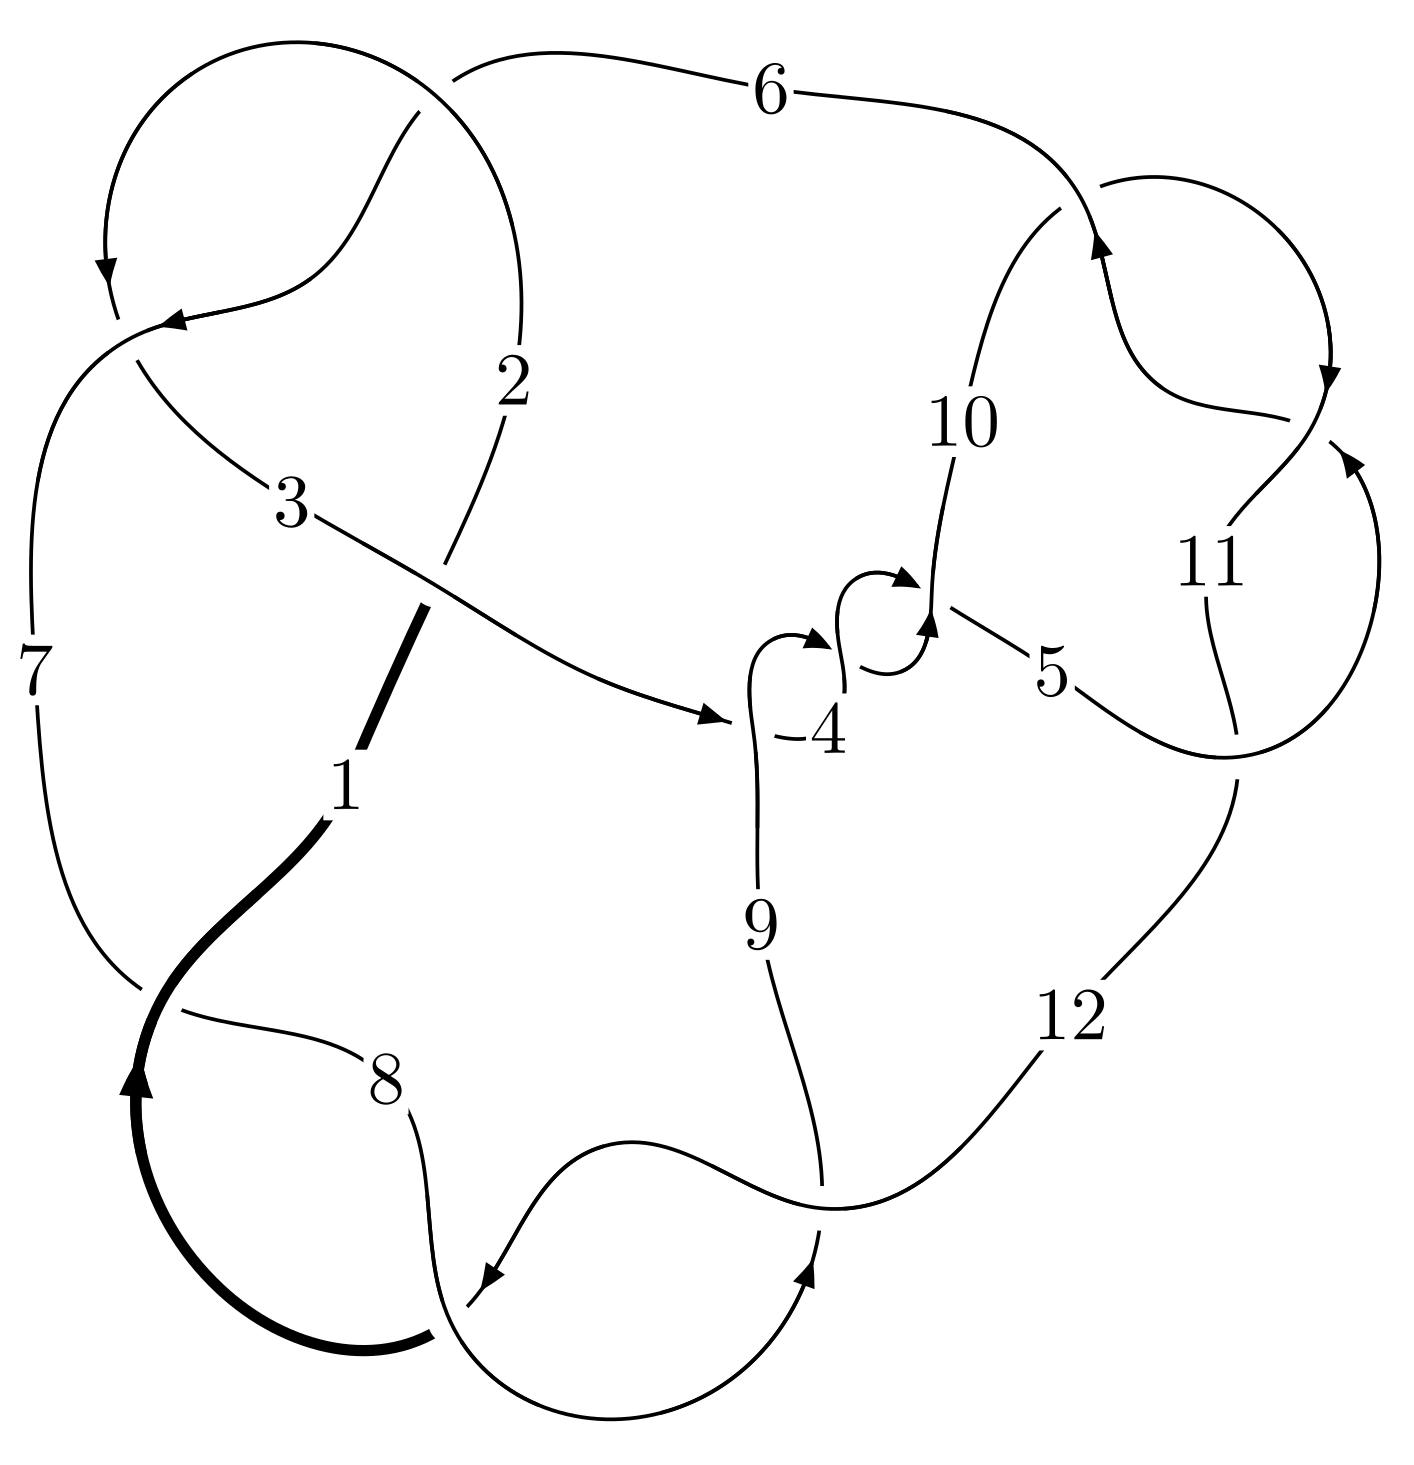
\includegraphics[width=112pt]{../../../GIT/diagram.site/Diagrams/png/1382_12a_0581.png}\\
\ \ \ A knot diagram\footnotemark}&
\allowdisplaybreaks
\textbf{Linearized knot diagam} \\
\cline{2-2}
 &
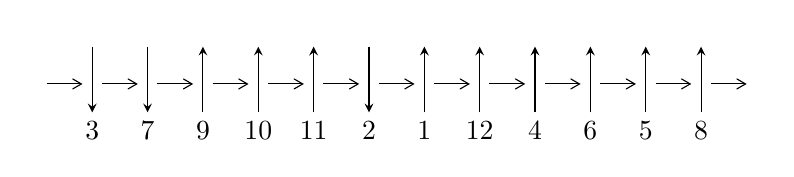
\begin{tikzpicture}[x=20pt, y=17pt]
	% nodes
	\node (C0) at (0, 0) {};
	\node (C1) at (1, 0) {};
	\node (C1U) at (1, +1) {};
	\node (C1D) at (1, -1) {3};

	\node (C2) at (2, 0) {};
	\node (C2U) at (2, +1) {};
	\node (C2D) at (2, -1) {7};

	\node (C3) at (3, 0) {};
	\node (C3U) at (3, +1) {};
	\node (C3D) at (3, -1) {9};

	\node (C4) at (4, 0) {};
	\node (C4U) at (4, +1) {};
	\node (C4D) at (4, -1) {10};

	\node (C5) at (5, 0) {};
	\node (C5U) at (5, +1) {};
	\node (C5D) at (5, -1) {11};

	\node (C6) at (6, 0) {};
	\node (C6U) at (6, +1) {};
	\node (C6D) at (6, -1) {2};

	\node (C7) at (7, 0) {};
	\node (C7U) at (7, +1) {};
	\node (C7D) at (7, -1) {1};

	\node (C8) at (8, 0) {};
	\node (C8U) at (8, +1) {};
	\node (C8D) at (8, -1) {12};

	\node (C9) at (9, 0) {};
	\node (C9U) at (9, +1) {};
	\node (C9D) at (9, -1) {4};

	\node (C10) at (10, 0) {};
	\node (C10U) at (10, +1) {};
	\node (C10D) at (10, -1) {6};

	\node (C11) at (11, 0) {};
	\node (C11U) at (11, +1) {};
	\node (C11D) at (11, -1) {5};

	\node (C12) at (12, 0) {};
	\node (C12U) at (12, +1) {};
	\node (C12D) at (12, -1) {8};
	\node (C13) at (13, 0) {};

	% arrows
	\draw[->,>={angle 60}]
	(C0) edge (C1) (C1) edge (C2) (C2) edge (C3) (C3) edge (C4) (C4) edge (C5) (C5) edge (C6) (C6) edge (C7) (C7) edge (C8) (C8) edge (C9) (C9) edge (C10) (C10) edge (C11) (C11) edge (C12) (C12) edge (C13) ;	\draw[->,>=stealth]
	(C1U) edge (C1D) (C2U) edge (C2D) (C3D) edge (C3U) (C4D) edge (C4U) (C5D) edge (C5U) (C6U) edge (C6D) (C7D) edge (C7U) (C8D) edge (C8U) (C9D) edge (C9U) (C10D) edge (C10U) (C11D) edge (C11U) (C12D) edge (C12U) ;
	\end{tikzpicture} \\
\hhline{~~} \\& 
\textbf{Solving Sequence} \\ \cline{2-2} 
 &
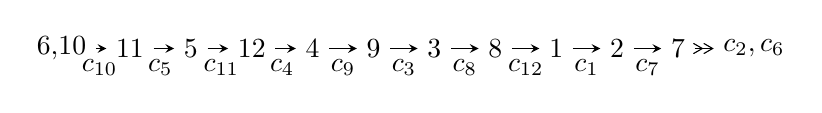
\begin{tikzpicture}[x=22pt, y=7pt]
	% node
	\node (A0) at (-1/8, 0) {6,10};
	\node (A1) at (1, 0) {11};
	\node (A2) at (2, 0) {5};
	\node (A3) at (3, 0) {12};
	\node (A4) at (4, 0) {4};
	\node (A5) at (5, 0) {9};
	\node (A6) at (6, 0) {3};
	\node (A7) at (7, 0) {8};
	\node (A8) at (8, 0) {1};
	\node (A9) at (9, 0) {2};
	\node (A10) at (10, 0) {7};
	\node (C1) at (1/2, -1) {$c_{10}$};
	\node (C2) at (3/2, -1) {$c_{5}$};
	\node (C3) at (5/2, -1) {$c_{11}$};
	\node (C4) at (7/2, -1) {$c_{4}$};
	\node (C5) at (9/2, -1) {$c_{9}$};
	\node (C6) at (11/2, -1) {$c_{3}$};
	\node (C7) at (13/2, -1) {$c_{8}$};
	\node (C8) at (15/2, -1) {$c_{12}$};
	\node (C9) at (17/2, -1) {$c_{1}$};
	\node (C10) at (19/2, -1) {$c_{7}$};
	\node (A11) at (45/4, 0) {$c_{2},c_{6}$};

	% edge
	\draw[->,>=stealth]	
	(A0) edge (A1) (A1) edge (A2) (A2) edge (A3) (A3) edge (A4) (A4) edge (A5) (A5) edge (A6) (A6) edge (A7) (A7) edge (A8) (A8) edge (A9) (A9) edge (A10) ;
	\draw[->>,>={angle 60}]	
	(A10) edge (A11);
\end{tikzpicture} \\ 

\end{tabular} \\

\footnotetext{
The image of knot diagram is generated by the software ``\textbf{Draw programme}" developed by Andrew Bartholomew(\url{http://www.layer8.co.uk/maths/draw/index.htm\#Running-draw}), where we modified some parts for our purpose(\url{https://github.com/CATsTAILs/LinksPainter}).
}\phantom \\ \newline 
\centering \textbf{Ideals for irreducible components\footnotemark of $X_{\text{par}}$} 
 
\begin{align*}
I^u_{1}&=\langle 
u^{59}+u^{58}+\cdots+3 u^2-1\rangle \\
\\
\end{align*}
\raggedright * 1 irreducible components of $\dim_{\mathbb{C}}=0$, with total 59 representations.\\
\footnotetext{All coefficients of polynomials are rational numbers. But the coefficients are sometimes approximated in decimal forms when there is not enough margin.}
\newpage
\renewcommand{\arraystretch}{1}
\centering \section*{I. $I^u_{1}= \langle u^{59}+u^{58}+\cdots+3 u^2-1 \rangle$}
\flushleft \textbf{(i) Arc colorings}\\
\begin{tabular}{m{7pt} m{180pt} m{7pt} m{180pt} }
\flushright $a_{6}=$&$\begin{pmatrix}0\\u\end{pmatrix}$ \\
\flushright $a_{10}=$&$\begin{pmatrix}1\\0\end{pmatrix}$ \\
\flushright $a_{11}=$&$\begin{pmatrix}1\\- u^2\end{pmatrix}$ \\
\flushright $a_{5}=$&$\begin{pmatrix}- u\\u^3+u\end{pmatrix}$ \\
\flushright $a_{12}=$&$\begin{pmatrix}u^2+1\\- u^4-2 u^2\end{pmatrix}$ \\
\flushright $a_{4}=$&$\begin{pmatrix}- u^3-2 u\\u^3+u\end{pmatrix}$ \\
\flushright $a_{9}=$&$\begin{pmatrix}- u^6-3 u^4-2 u^2+1\\u^6+2 u^4+u^2\end{pmatrix}$ \\
\flushright $a_{3}=$&$\begin{pmatrix}u^9+4 u^7+5 u^5-3 u\\- u^9-3 u^7-3 u^5+u\end{pmatrix}$ \\
\flushright $a_{8}=$&$\begin{pmatrix}u^{12}+5 u^{10}+9 u^8+4 u^6-6 u^4-5 u^2+1\\- u^{14}-6 u^{12}-13 u^{10}-10 u^8+4 u^6+8 u^4+u^2\end{pmatrix}$ \\
\flushright $a_{1}=$&$\begin{pmatrix}u^{22}+9 u^{20}+\cdots-2 u^2+1\\- u^{24}-10 u^{22}+\cdots-4 u^4-2 u^2\end{pmatrix}$ \\
\flushright $a_{2}=$&$\begin{pmatrix}u^{42}+17 u^{40}+\cdots-5 u^2+1\\- u^{42}-16 u^{40}+\cdots-12 u^4- u^2\end{pmatrix}$ \\
\flushright $a_{7}=$&$\begin{pmatrix}u^{32}+13 u^{30}+\cdots-8 u^2+1\\- u^{34}-14 u^{32}+\cdots+14 u^4+u^2\end{pmatrix}$\\&\end{tabular}
\flushleft \textbf{(ii) Obstruction class $= -1$}\\~\\
\flushleft \textbf{(iii) Cusp Shapes $= 4 u^{57}+4 u^{56}+\cdots+16 u+6$}\\~\\
\newpage\renewcommand{\arraystretch}{1}
\flushleft \textbf{(iv) u-Polynomials at the component}\newline \\
\begin{tabular}{m{50pt}|m{274pt}}
Crossings & \hspace{64pt}u-Polynomials at each crossing \\
\hline $$\begin{aligned}c_{1}\end{aligned}$$&$\begin{aligned}
&u^{59}+33 u^{58}+\cdots+6 u+1
\end{aligned}$\\
\hline $$\begin{aligned}c_{2},c_{6}\end{aligned}$$&$\begin{aligned}
&u^{59}- u^{58}+\cdots+2 u-1
\end{aligned}$\\
\hline $$\begin{aligned}c_{3},c_{4},c_{9}\end{aligned}$$&$\begin{aligned}
&u^{59}- u^{58}+\cdots-20 u-17
\end{aligned}$\\
\hline $$\begin{aligned}c_{5},c_{10},c_{11}\end{aligned}$$&$\begin{aligned}
&u^{59}+u^{58}+\cdots+3 u^2-1
\end{aligned}$\\
\hline $$\begin{aligned}c_{7},c_{8},c_{12}\end{aligned}$$&$\begin{aligned}
&u^{59}-3 u^{58}+\cdots-2 u+1
\end{aligned}$\\
\hline
\end{tabular}\\~\\
\newpage\renewcommand{\arraystretch}{1}
\flushleft \textbf{(v) Riley Polynomials at the component}\newline \\
\begin{tabular}{m{50pt}|m{274pt}}
Crossings & \hspace{64pt}Riley Polynomials at each crossing \\
\hline $$\begin{aligned}c_{1}\end{aligned}$$&$\begin{aligned}
&y^{59}-13 y^{58}+\cdots-18 y-1
\end{aligned}$\\
\hline $$\begin{aligned}c_{2},c_{6}\end{aligned}$$&$\begin{aligned}
&y^{59}-33 y^{58}+\cdots+6 y-1
\end{aligned}$\\
\hline $$\begin{aligned}c_{3},c_{4},c_{9}\end{aligned}$$&$\begin{aligned}
&y^{59}-53 y^{58}+\cdots-2694 y-289
\end{aligned}$\\
\hline $$\begin{aligned}c_{5},c_{10},c_{11}\end{aligned}$$&$\begin{aligned}
&y^{59}+47 y^{58}+\cdots+6 y-1
\end{aligned}$\\
\hline $$\begin{aligned}c_{7},c_{8},c_{12}\end{aligned}$$&$\begin{aligned}
&y^{59}+59 y^{58}+\cdots+94 y-1
\end{aligned}$\\
\hline
\end{tabular}\\~\\
\newpage\flushleft \textbf{(vi) Complex Volumes and Cusp Shapes}
$$\begin{array}{c|c|c}  
\text{Solutions to }I^u_{1}& \I (\text{vol} + \sqrt{-1}CS) & \text{Cusp shape}\\
 \hline 
\begin{aligned}
u &= \phantom{-}0.058378 + 1.130960 I\end{aligned}
 & -2.04129 + 1.77189 I & \phantom{-0.000000 } 0 \\ \hline\begin{aligned}
u &= \phantom{-}0.058378 - 1.130960 I\end{aligned}
 & -2.04129 - 1.77189 I & \phantom{-0.000000 } 0 \\ \hline\begin{aligned}
u &= -0.847163 + 0.084618 I\end{aligned}
 & -1.74912 - 9.58388 I & \phantom{-}5.65604 + 6.28826 I \\ \hline\begin{aligned}
u &= -0.847163 - 0.084618 I\end{aligned}
 & -1.74912 + 9.58388 I & \phantom{-}5.65604 - 6.28826 I \\ \hline\begin{aligned}
u &= \phantom{-}0.848749 + 0.035449 I\end{aligned}
 & \phantom{-}5.75598 + 5.05092 I & \phantom{-}9.97613 - 6.12158 I \\ \hline\begin{aligned}
u &= \phantom{-}0.848749 - 0.035449 I\end{aligned}
 & \phantom{-}5.75598 - 5.05092 I & \phantom{-}9.97613 + 6.12158 I \\ \hline\begin{aligned}
u &= -0.844748 + 0.015661 I\end{aligned}
 & \phantom{-}6.96091 - 0.69784 I & \phantom{-}12.84524 - 0.01265 I \\ \hline\begin{aligned}
u &= -0.844748 - 0.015661 I\end{aligned}
 & \phantom{-}6.96091 + 0.69784 I & \phantom{-}12.84524 + 0.01265 I \\ \hline\begin{aligned}
u &= \phantom{-}0.839398 + 0.078837 I\end{aligned}
 & \phantom{-}1.60637 + 4.73223 I & \phantom{-}8.74881 - 3.21994 I \\ \hline\begin{aligned}
u &= \phantom{-}0.839398 - 0.078837 I\end{aligned}
 & \phantom{-}1.60637 - 4.73223 I & \phantom{-}8.74881 + 3.21994 I \\ \hline\begin{aligned}
u &= -0.829147 + 0.087395 I\end{aligned}
 & -2.39103 - 0.42285 I & \phantom{-}4.73097 + 0.13131 I \\ \hline\begin{aligned}
u &= -0.829147 - 0.087395 I\end{aligned}
 & -2.39103 + 0.42285 I & \phantom{-}4.73097 - 0.13131 I \\ \hline\begin{aligned}
u &= \phantom{-}0.795102\phantom{ +0.000000I}\end{aligned}
 & \phantom{-}2.32839\phantom{ +0.000000I} & \phantom{-}4.51790\phantom{ +0.000000I} \\ \hline\begin{aligned}
u &= -0.371549 + 1.173570 I\end{aligned}
 & -5.71912 - 3.91206 I & \phantom{-0.000000 } 0 \\ \hline\begin{aligned}
u &= -0.371549 - 1.173570 I\end{aligned}
 & -5.71912 + 3.91206 I & \phantom{-0.000000 } 0 \\ \hline\begin{aligned}
u &= \phantom{-}0.110941 + 1.236520 I\end{aligned}
 & -3.06428 + 1.85081 I & \phantom{-0.000000 } 0 \\ \hline\begin{aligned}
u &= \phantom{-}0.110941 - 1.236520 I\end{aligned}
 & -3.06428 - 1.85081 I & \phantom{-0.000000 } 0 \\ \hline\begin{aligned}
u &= -0.396405 + 1.182980 I\end{aligned}
 & -5.12049 + 5.11297 I & \phantom{-0.000000 } 0 \\ \hline\begin{aligned}
u &= -0.396405 - 1.182980 I\end{aligned}
 & -5.12049 - 5.11297 I & \phantom{-0.000000 } 0 \\ \hline\begin{aligned}
u &= \phantom{-}0.384434 + 1.189160 I\end{aligned}
 & -1.80148 - 0.32610 I & \phantom{-0.000000 } 0 \\ \hline\begin{aligned}
u &= \phantom{-}0.384434 - 1.189160 I\end{aligned}
 & -1.80148 + 0.32610 I & \phantom{-0.000000 } 0 \\ \hline\begin{aligned}
u &= -0.154739 + 1.285240 I\end{aligned}
 & -5.10187 - 5.52444 I & \phantom{-0.000000 } 0 \\ \hline\begin{aligned}
u &= -0.154739 - 1.285240 I\end{aligned}
 & -5.10187 + 5.52444 I & \phantom{-0.000000 } 0 \\ \hline\begin{aligned}
u &= \phantom{-}0.391966 + 1.238580 I\end{aligned}
 & \phantom{-}2.03937 - 0.59806 I & \phantom{-0.000000 } 0 \\ \hline\begin{aligned}
u &= \phantom{-}0.391966 - 1.238580 I\end{aligned}
 & \phantom{-}2.03937 + 0.59806 I & \phantom{-0.000000 } 0 \\ \hline\begin{aligned}
u &= -0.058596 + 1.302090 I\end{aligned}
 & -6.34517 + 0.28249 I & \phantom{-0.000000 } 0 \\ \hline\begin{aligned}
u &= -0.058596 - 1.302090 I\end{aligned}
 & -6.34517 - 0.28249 I & \phantom{-0.000000 } 0 \\ \hline\begin{aligned}
u &= -0.387543 + 1.257050 I\end{aligned}
 & \phantom{-}3.11544 - 3.72547 I & \phantom{-0.000000 } 0 \\ \hline\begin{aligned}
u &= -0.387543 - 1.257050 I\end{aligned}
 & \phantom{-}3.11544 + 3.72547 I & \phantom{-0.000000 } 0 \\ \hline\begin{aligned}
u &= \phantom{-}0.349231 + 1.275480 I\end{aligned}
 & -1.63836 + 4.11991 I & \phantom{-0.000000 } 0\\
 \hline 
 \end{array}$$\newpage$$\begin{array}{c|c|c}  
\text{Solutions to }I^u_{1}& \I (\text{vol} + \sqrt{-1}CS) & \text{Cusp shape}\\
 \hline 
\begin{aligned}
u &= \phantom{-}0.349231 - 1.275480 I\end{aligned}
 & -1.63836 - 4.11991 I & \phantom{-0.000000 } 0 \\ \hline\begin{aligned}
u &= -0.384823 + 1.282600 I\end{aligned}
 & \phantom{-}2.92232 - 5.11207 I & \phantom{-0.000000 } 0 \\ \hline\begin{aligned}
u &= -0.384823 - 1.282600 I\end{aligned}
 & \phantom{-}2.92232 + 5.11207 I & \phantom{-0.000000 } 0 \\ \hline\begin{aligned}
u &= \phantom{-}0.386365 + 1.297270 I\end{aligned}
 & \phantom{-}1.60085 + 9.48535 I & \phantom{-0.000000 } 0 \\ \hline\begin{aligned}
u &= \phantom{-}0.386365 - 1.297270 I\end{aligned}
 & \phantom{-}1.60085 - 9.48535 I & \phantom{-0.000000 } 0 \\ \hline\begin{aligned}
u &= -0.126651 + 1.360960 I\end{aligned}
 & -9.41765 - 3.50298 I & \phantom{-0.000000 } 0 \\ \hline\begin{aligned}
u &= -0.126651 - 1.360960 I\end{aligned}
 & -9.41765 + 3.50298 I & \phantom{-0.000000 } 0 \\ \hline\begin{aligned}
u &= \phantom{-}0.476903 + 0.415250 I\end{aligned}
 & -7.45872 + 6.23445 I & \phantom{-}1.86893 - 7.19389 I \\ \hline\begin{aligned}
u &= \phantom{-}0.476903 - 0.415250 I\end{aligned}
 & -7.45872 - 6.23445 I & \phantom{-}1.86893 + 7.19389 I \\ \hline\begin{aligned}
u &= \phantom{-}0.441341 + 0.448361 I\end{aligned}
 & -7.59241 - 2.90093 I & \phantom{-}1.279113 - 0.509070 I \\ \hline\begin{aligned}
u &= \phantom{-}0.441341 - 0.448361 I\end{aligned}
 & -7.59241 + 2.90093 I & \phantom{-}1.279113 + 0.509070 I \\ \hline\begin{aligned}
u &= \phantom{-}0.118145 + 1.368160 I\end{aligned}
 & -13.24570 - 1.08745 I & \phantom{-0.000000 } 0 \\ \hline\begin{aligned}
u &= \phantom{-}0.118145 - 1.368160 I\end{aligned}
 & -13.24570 + 1.08745 I & \phantom{-0.000000 } 0 \\ \hline\begin{aligned}
u &= \phantom{-}0.134795 + 1.367180 I\end{aligned}
 & -13.0323 + 8.2643 I & \phantom{-0.000000 } 0 \\ \hline\begin{aligned}
u &= \phantom{-}0.134795 - 1.367180 I\end{aligned}
 & -13.0323 - 8.2643 I & \phantom{-0.000000 } 0 \\ \hline\begin{aligned}
u &= \phantom{-}0.375249 + 1.324440 I\end{aligned}
 & -2.78863 + 9.10055 I & \phantom{-0.000000 } 0 \\ \hline\begin{aligned}
u &= \phantom{-}0.375249 - 1.324440 I\end{aligned}
 & -2.78863 - 9.10055 I & \phantom{-0.000000 } 0 \\ \hline\begin{aligned}
u &= -0.368450 + 1.327520 I\end{aligned}
 & -6.82502 - 4.73394 I & \phantom{-0.000000 } 0 \\ \hline\begin{aligned}
u &= -0.368450 - 1.327520 I\end{aligned}
 & -6.82502 + 4.73394 I & \phantom{-0.000000 } 0 \\ \hline\begin{aligned}
u &= -0.378790 + 1.328850 I\end{aligned}
 & -6.1782 - 13.9904 I & \phantom{-0.000000 } 0 \\ \hline\begin{aligned}
u &= -0.378790 - 1.328850 I\end{aligned}
 & -6.1782 + 13.9904 I & \phantom{-0.000000 } 0 \\ \hline\begin{aligned}
u &= -0.445899 + 0.414347 I\end{aligned}
 & -3.89834 - 1.60598 I & \phantom{-}4.85193 + 4.07841 I \\ \hline\begin{aligned}
u &= -0.445899 - 0.414347 I\end{aligned}
 & -3.89834 + 1.60598 I & \phantom{-}4.85193 - 4.07841 I \\ \hline\begin{aligned}
u &= -0.451600 + 0.225417 I\end{aligned}
 & -0.51874 - 3.38908 I & \phantom{-}6.72883 + 9.41856 I \\ \hline\begin{aligned}
u &= -0.451600 - 0.225417 I\end{aligned}
 & -0.51874 + 3.38908 I & \phantom{-}6.72883 - 9.41856 I \\ \hline\begin{aligned}
u &= -0.171695 + 0.376972 I\end{aligned}
 & -1.43291 + 1.09097 I & \phantom{-}0.441701 - 0.484421 I \\ \hline\begin{aligned}
u &= -0.171695 - 0.376972 I\end{aligned}
 & -1.43291 - 1.09097 I & \phantom{-}0.441701 + 0.484421 I \\ \hline\begin{aligned}
u &= \phantom{-}0.404352 + 0.062637 I\end{aligned}
 & \phantom{-}0.771139 + 0.080818 I & \phantom{-}13.47182 - 1.34489 I \\ \hline\begin{aligned}
u &= \phantom{-}0.404352 - 0.062637 I\end{aligned}
 & \phantom{-}0.771139 - 0.080818 I & \phantom{-}13.47182 + 1.34489 I\\
 \hline 
 \end{array}$$\newpage
\newpage\renewcommand{\arraystretch}{1}
\centering \section*{ II. u-Polynomials}
\begin{tabular}{m{50pt}|m{274pt}}
Crossings & \hspace{64pt}u-Polynomials at each crossing \\
\hline $$\begin{aligned}c_{1}\end{aligned}$$&$\begin{aligned}
&u^{59}+33 u^{58}+\cdots+6 u+1
\end{aligned}$\\
\hline $$\begin{aligned}c_{2},c_{6}\end{aligned}$$&$\begin{aligned}
&u^{59}- u^{58}+\cdots+2 u-1
\end{aligned}$\\
\hline $$\begin{aligned}c_{3},c_{4},c_{9}\end{aligned}$$&$\begin{aligned}
&u^{59}- u^{58}+\cdots-20 u-17
\end{aligned}$\\
\hline $$\begin{aligned}c_{5},c_{10},c_{11}\end{aligned}$$&$\begin{aligned}
&u^{59}+u^{58}+\cdots+3 u^2-1
\end{aligned}$\\
\hline $$\begin{aligned}c_{7},c_{8},c_{12}\end{aligned}$$&$\begin{aligned}
&u^{59}-3 u^{58}+\cdots-2 u+1
\end{aligned}$\\
\hline
\end{tabular}\newpage\renewcommand{\arraystretch}{1}
\centering \section*{ III. Riley Polynomials}
\begin{tabular}{m{50pt}|m{274pt}}
Crossings & \hspace{64pt}Riley Polynomials at each crossing \\
\hline $$\begin{aligned}c_{1}\end{aligned}$$&$\begin{aligned}
&y^{59}-13 y^{58}+\cdots-18 y-1
\end{aligned}$\\
\hline $$\begin{aligned}c_{2},c_{6}\end{aligned}$$&$\begin{aligned}
&y^{59}-33 y^{58}+\cdots+6 y-1
\end{aligned}$\\
\hline $$\begin{aligned}c_{3},c_{4},c_{9}\end{aligned}$$&$\begin{aligned}
&y^{59}-53 y^{58}+\cdots-2694 y-289
\end{aligned}$\\
\hline $$\begin{aligned}c_{5},c_{10},c_{11}\end{aligned}$$&$\begin{aligned}
&y^{59}+47 y^{58}+\cdots+6 y-1
\end{aligned}$\\
\hline $$\begin{aligned}c_{7},c_{8},c_{12}\end{aligned}$$&$\begin{aligned}
&y^{59}+59 y^{58}+\cdots+94 y-1
\end{aligned}$\\
\hline
\end{tabular}
\vskip 2pc
\end{document}